\section*{Цель работы}
Изучить принцип работы регистров сдвига и дешифраторов с использованием среды Verilog, проанализировать их RTL интерпретации и временные диаграммы.

\section*{ \fbox{ Задание 1. } }
\begin{quote}
    {\itshape
        Собрать схему четырехразрядного регистра сдвига. Изучить схему, реализованную в RTL-Viewer. Построить временные диаграммы, иллюстрирующие работу устройства. Период тактового сигнала задать 25 нс.

        Изменить код программы. Открыть полученную схему в RTL-Viewer, построить временные диаграммы. Что изменилось в схеме, почему?
    }
\end{quote}

\begin{codemultipage}
    \captionof{listing}{Регистр сдвига\label{lst:sdvig.v}}
    \nopagebreak
    \inputminted{verilog}{scripts/sdvig.v}
\end{codemultipage}
\begin{codemultipage}
    \captionof{listing}{Регистр сдвига неправильный\label{lst:sdvig_wrong.v}}
    \nopagebreak
    \inputminted{verilog}{scripts/sdvig_wrong.v}
\end{codemultipage}

\begin{figure}[H]
    \centering
    \includegraphics[width=1\textwidth]{figs/sdvig_RTL.pdf}
    \caption{Регистр сдвига --- RTL.}
    \label{fig:sdvig_RTL.pdf}
\end{figure}
\begin{figure}[H]
    \centering
    \includegraphics[width=0.5\textwidth]{figs/sdvig_wrong_RTL.pdf}
    \caption{Регистр сдвига неправильный --- RTL.}
    \label{fig:sdvig_wrong_RTL.pdf}
\end{figure}

\begin{figure}[H]
    \centering

    \begin{subfigure}[c]{0.48\textwidth}
        \centering
        \includegraphics[width=\textwidth]{figs/sdvig_vwf_func.png}
        \caption{Functional}
        \label{fig:sdvig_vwf_func}
    \end{subfigure}
    \hfill
    \begin{subfigure}[c]{0.48\textwidth}
        \centering
        \includegraphics[width=\textwidth]{figs/sdvig_vwf_time.png}
        \caption{Timing}
        \label{fig:sdvig_vwf_time}
    \end{subfigure}

    \caption{Регистр сдвига --- временная диаграмма.}
    \label{fig:sdvig_vwf}
\end{figure}

\begin{figure}[H]
    \centering

    \begin{subfigure}[c]{0.48\textwidth}
        \centering
        \includegraphics[width=\textwidth]{figs/sdvig_wrong_vwf_func.png}
        \caption{Functional}
        \label{fig:sdvig_wrong_vwf_func}
    \end{subfigure}
    \hfill
    \begin{subfigure}[c]{0.48\textwidth}
        \centering
        \includegraphics[width=\textwidth]{figs/sdvig_wrong_vwf_time.png}
        \caption{Timing}
        \label{fig:sdvig_wrong_vwf_time}
    \end{subfigure}

    \caption{Регистр сдвига неправильный --- временная диаграмма.}
    \label{fig:sdvig_wrong_vwf}
\end{figure}

\subsection*{Анализ регистра сдвига}
RTL схема регистра представлена на \cref{fig:sdvig_RTL.pdf}. Проанализируем её.
На схеме пресдставлены уже известные элементы из предыдущих лабораторных работ: мультиплексоры, D-триггеры.

Из схемы хорошо видно, что входной сигнал clock подается в соответствующие входы в триггерах, следовательно они синхронны (что подтверждается кодом).

Проследим за воздействием load. Оно подается на входы SEL мультиплексоров, которые на свой выход подают сигнал со входа 0, если $\text{load}=0$, и со входа 1, если $\text{load}=1$.

Проследим за входами 1 у мультиплексоров. Все они подсоединены ко входному сигналу data\_in, а значит во время истинности load мультиплексоры просто передают data\_in на своих выходы.

Выходы мультиплексоров всегда ведут в соответствующие входы триггеров. Таким образом истинность load просто перезаписывает все триггеры в соответствии с сигналом data\_in. Это хорошо видно из временной диаграммы на \cref{fig:sdvig_vwf}: $\text{data\_in}=1_{10}=0001_2 \implies (\text{qa},\text{qb},\text{qc},\text{qd})=(0,0,0,1)$.

Проанализируем случай, когда load ложен. В таком случае сигналы с триггеров qa, qb, qc, qd передаются в триггеры qb, qc, qd, qa соответственно. Таким образом происходит сдвиг сигнала с каждым тактом. Действительно, именно этот процесс отражает \cref{fig:sdvig_vwf}.

\subsection*{Анализ регистра сдвига неправильного}
RTL схема на \cref{fig:sdvig_wrong_RTL.pdf} существенно отличается от предыдущей. Во-первых здесь отсутствуют мультиплексоры; во-вторых нет обмена значениями триггеров между собой.

Проследим за логикой. Тактовый сигнал корректно изображен согласно теоретическим представлениям о нем. Входно йсигнал ds напрямую приходит ко входам каждого триггера. Таким образом с каждым рабочим тактом сигнал ds просто перезаписывает все триггеры, что существенно отличается от логики правильного регистра сдвига.

Проанализируем код неправильного регистра \cref{lst:sdvig_wrong.v} и сравним его с правильным \cref{lst:sdvig.v}. Сразу заметно отличие сигнала load. Логику неправильного регистра можно интерпретировать, как будто load всегда истиннен. Код на строках 7--10 нерправильного регистра, кажется, соответствует коду на строках 17--20 правильного за одним исключением: присваивание сигнала происходит не через оператор \mintinline{text}§<=§, а через оператор \mintinline{text}§=§.

Обратимся к документации Verilog.
\begin{itemize}
    \item Оператор \mintinline{text}§=§ называется блокирующим присваиванием. Срабатывает немедленно, подобно классическим языкам программирования (напр. С): следующая строка кода не выполнится, пока присваивание не завершится.
    \item Оператор \mintinline{text}§<=§ называется неблокирующим присваиванием. Срабатывает одновременно с остальными такими же операторами: все правые части выражений вычисляются одновременно в начале шага симуляции, а значения в левых частях обновляются только в конце шага.
\end{itemize}
Здесь вспоминается и раскрывается подвывод, к которому привела предыдущая лабораторная работа №5:
\begin{quote}
    {\itshape
        <...> особенность языка Verilog.
        Он является не столько языком программирования, сколько языком описания схем. Поэтому последовательность строк <...> не имеет значения --- состояние обоих переменных обновляется одновременно в момент времени <...>.
    }
\end{quote}
Оператор неблокирующего присваивания является нативным для Verilog и соответствует его <<описательной>> логике, а блокирующее присванивание наследуется из классических <<директивных>> языков программирования. Именно это важное отличие и объясняет неправильную работу неправильного регистра сдвига.



\section*{ \fbox{ Задание 2. } }
\begin{quote}
    {\itshape
        Собрать схему дешифратора $2\times4$, тип 2 (дешифратор --- схема преобразования двоичного кода в унитарный). Изучить схему, реализованную в RTL-Viewer. Построить временные диаграммы, иллюстрирующие работу устройства. Период входного сигнала задать 30 нс.
    }
\end{quote}

\begin{codemultipage}
    \captionof{listing}{Дешифратор, тип 2.\label{lst:dc2.v}}
    \nopagebreak
    \inputminted{verilog}{scripts/dc2.v}
\end{codemultipage}

\begin{figure}[H]
    \centering
    \includegraphics[width=0.6\textwidth]{figs/dc2_RTL.pdf}
    \caption{Дешифратор, тип 2 --- RTL.}
    \label{fig:dc2_RTL.pdf}
\end{figure}

\begin{figure}[H]
    \centering

    \begin{subfigure}[c]{0.48\textwidth}
        \centering
        \includegraphics[width=\textwidth]{figs/dc2_vwf_func.png}
        \caption{Functional}
        \label{fig:dc2_vwf_func}
    \end{subfigure}
    \hfill
    \begin{subfigure}[c]{0.48\textwidth}
        \centering
        \includegraphics[width=\textwidth]{figs/dc2_vwf_time.png}
        \caption{Timing}
        \label{fig:dc2_vwf_time}
    \end{subfigure}

    \caption{Дешифратор, тип 2 --- временная диаграмма.}
    \label{fig:dc2_vwf}
\end{figure}

\subsection*{Анализ RTL схемы}
RTL схема на \cref{fig:dc2_RTL.pdf} проста, однако на ней есть новый элемент, называемый LEFT\_SHIFT или логический сдвиг влево. Изучим его.

Логический сдвиг влево имеет два входа и один выход. Выход является результатом работы сдвига. Наибольший интерес для нас представляют входы \mintinline{text}§32'h00000001§ и \mintinline{text}§COUNT[1..0]§ (назовем их сигналами сдвига и данных соответсвенно). Вход сдвига соответсвует 32-х битному числу, значение которого равно единице.

Для того, чтобы понять, как именно работает элемент сдвига, обратимся к \cref{lst:dc2.v,fig:dc2_vwf}. Из временной диаграммы видно, что десятичное значение сигнала in отражает какой по счету бит сигнала out будет истиннен. Из кода видно, что в out блокирующе присваивается однобитная единица, которая сдвинута влево на число разрядов, равное числу in.

Таким образом логика элмента сдвига становится ясной. Она побитно сдвигает свой первый вход на число знаков, равное числу второго входа.

\section*{ \fbox{ Задание 3. } }
\begin{quote}
    {\itshape
        Собрать схему дешифратора двоичного кода в код семисегментного индикатора. Самостоятельно дописать коды символов с D по F.

        Изучить работу схемы в RTL Viever. Как работает дешифратор и на каких элементах он основан? Зачем нужен сигнал dig? Какой индикатор используется в задании, с общим катодом или с общим анодом?
    }
\end{quote}

\begin{figure}[H]
    \centering
    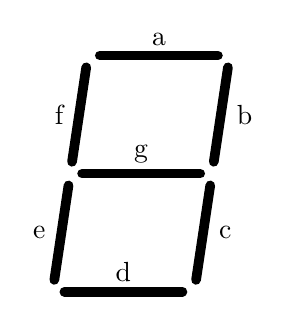
\begin{tikzpicture}[
        scale = 1.5,
        % Наклон всей фигуры (xslant)
        xslant=0.15, 
        % Стиль для сегментов: цвет, толщина и скругленные концы
        segment/.style={
            line width=3.5pt, 
            line cap=round
        },
        % Стиль для буквенных меток
        label style/.style={
            black, 
            % font=\sffamily\small,
            inner sep=2pt
        }
    ]

        % Координаты для сетки (ширина 1.2, высота 2.2)
        % Горизонтальные сегменты
        \draw[segment] (0.1, 2) -- (1.1, 2) node[label style, midway, above] {a}; % a
        \draw[segment] (0.1, 1) -- (1.1, 1) node[label style, midway, above] {g}; % g
        \draw[segment] (0.1, 0) -- (1.1, 0) node[label style, midway, above] {d}; % d

        % Вертикальные сегменты (левая сторона)
        \draw[segment] (0, 1.1) -- (0, 1.9) node[label style, midway, left=2pt] {f};  % f
        \draw[segment] (0, 0.1) -- (0, 0.9) node[label style, midway, left=2pt] {e};  % e

        % Вертикальные сегменты (правая сторона)
        \draw[segment] (1.2, 1.1) -- (1.2, 1.9) node[label style, midway, right=2pt] {b}; % b
        \draw[segment] (1.2, 0.1) -- (1.2, 0.9) node[label style, midway, right=2pt] {c}; % c

    \end{tikzpicture}
    \caption{Обозначения сегментов}
    \label{fig:segments}
\end{figure}

\begin{codemultipage}
    \captionof{listing}{Дешифратор двоичного кода в код семисегментного индикатора\label{lst:seg7.v}}
    \nopagebreak
    \inputminted{verilog}{scripts/seg7.v}
\end{codemultipage}

\subsection*{Заполнение кодов символов D--F}
Из \cref{fig:segments} ясно видно за какой сегмент отвечает какой бит. Из строк 8--20 \cref{lst:seg7.v} ясно прослеживается логика: семибитное значение, описывающее символ, записывается как $7'b\boxed{g\mathstrut}\boxed{f\mathstrut}\boxed{e\mathstrut}\boxed{d\mathstrut}\boxed{c\mathstrut}\boxed{b\mathstrut}\boxed{a\mathstrut}$. Остается только вообразить то, какие сегменты должны гореть для каждой из букв на индикаторе и закодировать их соотвествующим образом, как на строках 21--23.

\begin{figure}[H]
    \centering
    \includegraphics[width=0.5\textwidth]{figs/seg7_RTL.pdf}
    \caption{Дешифратор двоичного кода в код семисегментного индикатора --- RTL.}
    \label{fig:seg7_RTL.pdf}
\end{figure}

\subsection*{Анализ RTL схемы}
RTL схема представлена на \cref{fig:seg7_RTL.pdf}. Ответим на вопросы.

\subsubsection*{Как работает дешифратор и на каких элементах он основан?}
На RTL схеме представлен новый элемент DECODER и ряд элементов ИЛИ. Количество элементов ИЛИ равно числу бит для индикатора --- семи $\left(\underset{7}{g\mathstrut} \underset{6}{f\mathstrut} \underset{5}{e\mathstrut} \underset{4}{d\mathstrut} \underset{3}{c\mathstrut} \underset{2}{b\mathstrut} \underset{1}{a\mathstrut}\right)$, следовательно они отвечают за логику отрисовки конкретного сегмента в индикаторе.

Для того, чтобы понять, зачем нужен и как работает элемент DECODER, проанализируем \cref{lst:seg7.v}. Из него ясно видно, что входным сигналом bcd кодируется символ, который следует отобразить на индикаторе. Примечательно и удобно, что символы соотвествуеют 16-ричной системе счисления. Итак, bcd является 4-х битным число и способно закодировать $2^4=16$ разных состояний. Действительно, выход DECODER out является 16-ти битным числом. Отсюда становится ясно, что DECODER просто декодирует десятичное число со входа и на выходе дает сигнал на соответсвующий по счету бит. Так, если вход $0010_2=2_{10}$, то выход
$
\underset{\scriptscriptstyle 16}{0} ~
\underset{\scriptscriptstyle 15}{0} ~
\underset{\scriptscriptstyle 14}{0} ~
\underset{\scriptscriptstyle 13}{0} \quad
\underset{\scriptscriptstyle 12}{0} ~
\underset{\scriptscriptstyle 11}{0} ~
\underset{\scriptscriptstyle 10}{0} ~
\underset{\scriptscriptstyle 9}{0} \quad
\underset{\scriptscriptstyle 8}{0} ~
\underset{\scriptscriptstyle 7}{0} ~
\underset{\scriptscriptstyle 6}{0} ~
\underset{\scriptscriptstyle 5}{0} \quad
\underset{\scriptscriptstyle 4}{0} ~
\underset{\scriptscriptstyle 3}{0} ~
\underset{\scriptscriptstyle 2}{1} ~
\underset{\scriptscriptstyle 1}{0}
$.

Выходной сигнал подобного вида подается на соответствующие входы элементов ИЛИ, они отрабатывают и в leds записывается значение, описанное на \cref{lst:seg7.v} на строках 8--23.

\subsubsection*{Зачем нужен сигнал dig?}
Индикаторы (\cref{fig:segments}) можно часто увидеть на калькуляторах или светофорах. На этих устройствах обычно записываются не просто цифра, а числа. Число состоит из набора цифр, каждая из которых должна располагаться на своем месте, называемом разрядом. Здесь становится понятно, что сигнал dig включает или отключает разряд, на котором должен отображаться данный индикатор. В данном случае dig является однобитным и постоянно равен 1, а значит наше устройство способно отображать только одну цифру и всегда ее выводит.

\subsubsection*{Какой индикатор используется в задании, с общим катодом или с общим анодом?}
Индикаторы разделяют с общим анодом и с общим катодом, их отличие заключается в следующем: зажигаем сегменты на индикаторы мы истинным сигналом или ложным. 

Посмотрим на строку \cref{lst:seg7.v} 8 для нуля. Бит $\text{g}=1$, а остальные равны нулю. Из \cref{fig:segments} видно, что бит g соотвествует центральному горизонтальному сегменту. Это значит, что единичным сигналом мы тушим сегменты, а значит данный индикатор с общим анодом.

\section*{ \fbox{ Задание 4. } }
\begin{quote}
    {\itshape
        К коду задания 3 добавить счетчик с управлением от кварцевого резонатора (50 МГц). Из всех выходов 32-разрядного счетчика для отображения информации взять q[29:26]. Какова частота смены состояний на индикаторе?
    }
\end{quote}

\begin{codemultipage}
    \captionof{listing}{Дешифратор с добавленным счетчиком\label{lst:freq.v}}
    \nopagebreak
    \inputminted{verilog}{scripts/freq.v}
\end{codemultipage}

\begin{figure}[H]
    \centering
    \includegraphics[width=0.75\textwidth]{figs/freq_RTL.pdf}
    \caption{Дешифратор с добавленным счетчиком --- RTL.}
    \label{fig:freq_RTL.pdf}
\end{figure}

\subsection*{Определение частоты состояний на индикаторе}
В лабораторной работе №5 уже была выведена формула для расчета частоты на конкретном бите:
\begin{equation}
    f_i
    = \frac{
        f_0
    }{
        2^{i + 1}
    }.
    \label{eq:fi}
\end{equation}

Индикатор меняется при изменении самого младшего разряда, в данном случае это 26-ой бит. Посчитаем, как часто он меняет свое состояние:
\begin{equation}
    f_{26}
    = \frac{
        50 \cdot 10^6~Гц
    }{
        2^{26 + 1}
    }
    = \pv[.4]{50e6 / (2**(26 + 1))}~Гц.
    \label{eq:fic}
\end{equation}

Таким образом индикатор будет менять свое состояние раз в $t=\cfrac1{f_{26}}=\pv[.2]{1 / ( 50e6 / (2**(26 + 1)) )}~с$.

\section*{Выводы}

% === Отчет должен содержать:
% - текст программы
% - скриншоты из RTL-Viewer и временные диаграммы при наличии задержек
% - пояснения по заданным в задании вопросам. 


В ходе выполнения лабораторной работы были проанализированы RTL схемы и временные диаграммы регистров сдвига и дешифраторов.

Было выяснено, что для корректного выполнения регистра сдвига необходимо использовать неблокирующий оператор присваивания. Использование \mintinline{text}§=§ приводит к некорректной работе.

Дешифратор $2\times4$ работает за счет элемента левого сдвига. В Verilog данному элементу соответствует оператор \mintinline{text}§<<§.

Дешифратор двоичного кода в код семисегментного индикатора работает за счет элемнта DECODER и набора элеметов ИЛИ. Сигнал dig в подобных устройствах отражает, какой разряд следует отображать, а какой нет. Было установлено различие индикаторов с общим анодом и общим катодом.

Были выполнены расчеты для выяснения частоты смены состояний на индикаторе при тактовой частоте 50 МГц при условии, что для отображения информации берутся биты 29--26.
